\section{Relasjonsskjema}

\subsection{Tabeller}

\vspace{0.3cm}

\sqlcolumns{users}

\begin{itemize}
    \item Primærnøkkel er \verb|user_email| (brukerens epost-adresse, naturlig nøkkel).
    \item Tabellen er på 4NF.
    \begin{itemize}
        \item Alle attributter er atomiske (1NF)
        \item \verb|user_email| er eneste nøkkelattributt (2NF)
        \item Det er ingen transitive avhengigheter (3NF)
        \item Alle avhengigheter har \verb|user_email| på venstre side (BCNF)
        \item \verb|user_email| gir aldri mer enn én verdi uansett hvilke kolonner som velges (4NF) 
    \end{itemize}
\end{itemize}

\vspace{0.5cm}

\sqlcolumns{reviews}

\begin{itemize}
    \item Primærnøkkel er \verb|review_id| (generert nøkkel).
    \item \verb|user_email| og \verb|coffee_id| er fremmednøkler til hhv. \class{users} og \class{coffee}.
    \item Tabellen er på 4NF.
    \begin{itemize}
        \item Alle attributter er atomiske (1NF)
        \item Ikke-nøkkelattributtene er kun funksjonelt avhengig av hele kandidatnøkler (2NF)
        \begin{itemize}
            \item Ikke-nøkkelattributtene er \verb|rating| og \verb|note|
            \item Kandidatnøklene er \verb|review_id| og (\verb|user_email|, \verb|coffee_id|, \verb|date_time|)
        \end{itemize}
        \item Det er ingen funksjonelle avhengigheter mellom ikke-nøkkelattributter (3NF)
        \item Alle avhengigheter har en supernøkkel på venstre side av avhengigheten (BCNF)
        \item En vilkårlig supernøkkel gir maks én mulig verdi for samtlige kolonner (4NF)
    \end{itemize}
\end{itemize}

\pagebreak

\sqlcolumns{coffee}

\begin{itemize}
    \item Primærnøkkel er \verb|coffee_id| (generert nøkkel).
    \item \verb|roastery_name| er fremmednøkkel til \class{roasteries}.
    \item Tabellen er på 4NF.
    \begin{itemize}
        \item Attributtene er atomiske (1NF)
        \item Alle avhengigher har hele kandidatnøkler på venstre side (2NF, 3NF, BCNF)
        \item \begin{itemize}
            \item Kandidatnøklene er \verb|coffee_id| og (\verb|coffee_name|, \verb|roastery_name|)
        \end{itemize}
        \item Ingen supernøkler gir mer enn én verdi for en vilkårlig kolonne (4NF)
    \end{itemize}
\end{itemize}

\vspace{0.7cm}

\sqlcolumns{farms}

\begin{itemize}
    \item Primærnøkkel er \verb|farm_name| (gårdsnavn, naturlig nøkkel).
    \item Tabellen er på 4NF.
    \begin{itemize}
        \item Attributtene er atomiske (1NF)
        \item \verb|farm_name| er på venstre side av alle avhengigheter (2NF, 3NF, BCNF)
        \begin{itemize}
            \item Vi antar at region ikke entydig gir land (land kan ha regioner som deler navn)
        \end{itemize}
        \item \verb|farm_name| gir en-og-bare-en verdi for alle kolonner (4NF)
    \end{itemize}
\end{itemize}

\vspace{0.7cm}

\sqlcolumns{batches}

\begin{itemize}
    \item Primærnøkkel er \verb|batch_id| (generert nøkkel).
    \item Fremmednøkler:
    \begin{itemize}
        \item \verb|coffee_id| \rightarrow \ \class{coffee}
        \item \verb|roastery_name| \rightarrow \ \class{roasteries}
        \item \verb|farm_name| \rightarrow \ \class{farms}
        \item \verb|refinement_name| \rightarrow \ \textbf{\ttfamily refinement\_methods}
    \end{itemize}
    \pagebreak
    \item Tabellen er på 4NF.
    \begin{itemize}
        \item Attributtene er atomiske (1NF) og ingen nøkler er sammensatte (2NF)
        \item Alle funksjonelle avhengigheter har en supernøkkel på venstre side (3NF, BCNF)
        \item Supernøkler gir maks én verdi for alle kolonner (4NF)
    \end{itemize}
\end{itemize}

\vspace{0.5cm}

\sqlcolumns{refinement_methods}

\begin{itemize}
    \item Primærnøkkel er \verb|refinement_name| (navn på foredlingsmetode, naturlig nøkkel).
    \item Tabellen er på 4NF.
    \begin{itemize}
        \item Attributtene er atomiske (1NF)
        \item Eneste funksjonelle avhengighet er \verb|refinement_method| \rightarrow \ \verb|refinement_description| (2NF, 3NF, BCNF).
        \item Tabellen er 2D og BCNF (4NF)
    \end{itemize}
\end{itemize}

\vspace{0.2cm}

Følgende tabeller er 4NF fordi attributtene er atomiske (1NF) og består av to kolonner som begge er nøkler (2NF, 3NF, BCNF, 4NF).

\sqlcolumns{beans_in_batch}

\sqlcolumns{farm_cultivate_beans}

\vspace{-0.7cm}

\begin{itemize}
    \item (\verb|batch_id|, \verb|bean_type|) er sammensatt primærnøkkel i {\textbf{\ttfamily beans\_in\_batch}}.
    \begin{itemize}
        \item \verb|batch_id| og \verb|bean_type| er fremmednøkler til hhv. \class{batches} og {\textbf{\ttfamily coffee\_beans}}.
    \end{itemize}
    \item (\verb|farm_name|, \verb|bean_type|) er sammensatt primærnøkkel i {\textbf{\ttfamily farm\_cultivate\_beans}}.
    \begin{itemize}
        \item \verb|farm_name| og \verb|bean_type| er fremmednøkler til hhv. \class{farms} og {\textbf{\ttfamily coffee\_beans}}.
    \end{itemize}
\end{itemize}

Følgende tabeller har bare én dimensjon og er derfor ikke på normalform:

\sqlcolumns{roasteries}

\sqlcolumns{coffee_beans}

\begin{itemize}
    \item \verb|roastery_name| er primærnøkkel (navn på brenneri, naturlig nøkkel)
    \item \verb|bean_type| er primærnøkkel (navn på kaffebønne, naturlig nøkkel)
\end{itemize}

\pagebreak

\subsection{Diagram}

\vspace{1cm}

\makebox[\textwidth][c]{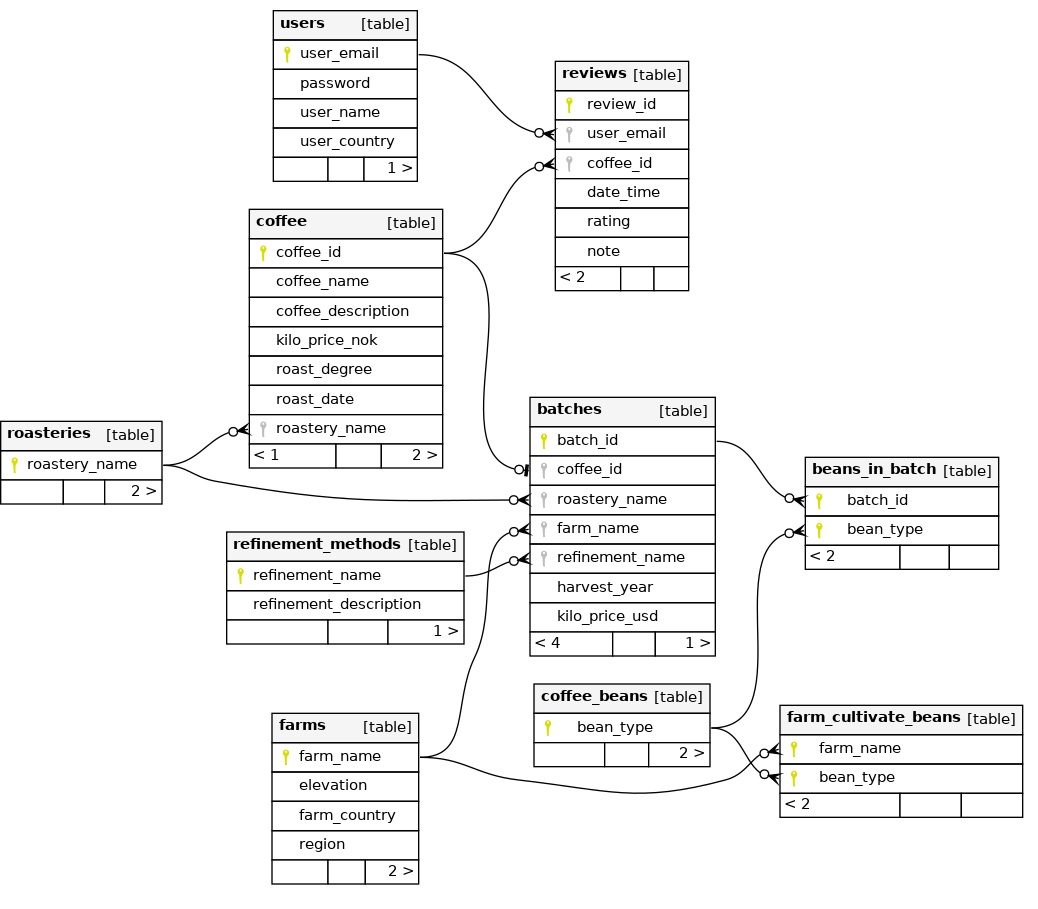
\includegraphics[width=1.2\textwidth]{schemaspy.png}}